\documentclass[conference]{IEEEtran}
\usepackage[colorlinks,allcolors=blue]{hyperref}
\usepackage{amsfonts}
\usepackage{graphicx}

\graphicspath{{./images/}}


\begin{document}

    \title{Modeling and Observing ProtoDigital Twin with ROS2 and Omniverse}
    \author{\IEEEauthorblockN{Alican Tüzün} 
    \IEEEauthorblockA{University of Applied Sciences Upper Austria\\ Wels, Austria\\ tuzunalican@gmail.com\\}}
    
    \maketitle

    \begin{abstract}
        Digital twins are becoming more and more important for the efficient and effective development and operation of cyber-physical systems.
        However, digital twins are only useful if they reflect the real-world system accurately enough, i.e.their quality is high enough. 
        This claim entails the question, of what the term quality in the context of digital twins means and how it can be measured. 
        In this article, we present our experience with the quality assurance of a digital twin for an assembly line in the automotive industry.
        We explain our preliminary definition of digital twin quality, which we derive from classical quality models for general software systems. 
        Furthermore, we describe quality issues, which we were able to detect in a digital twin of an assembly line in the automotive industry. \
        Finally, we conclude how to leverage our experience in different contexts and how to generalize the underlying approaches.
    \end{abstract}

    \section{Introduction}\label{section:introduction}
    As new and complex technologies advance to emerge, it becomes progressively difficult to understand and define their core concepts.
    One of the significant current examples in the field of digitalization is the notion of digital twins, which has resulted in numerous definitions~\cite{Review1}, 
    that vary from one derivation to another. Because, even though the terms "digital" and "twin" are easy to grasp, their consolidation develops a new challenging concept, 
    which might be resulted in misunderstanding and misapplication. Therefore, a practical example of a proto, easy-to-model example of the digital twin prototype and instance 
    can significantly improve understanding of the notion of the digital twin.
    
    The digital twin (DT) was proposed in 2002 by Grieves~\cite{Originsofdigitaltwinconcept}, as an ideal form of product life cycle management. The proposal was to create a co-existed information twin of 
    a real system to gather new information to minimize the system needs and waste, such as material, time, and energy. It should be noted that initially this concept was called the mirrored spaced model~\cite{Originsofdigitaltwinconcept}, 
    and later the information mirroring model (IMM)~\cite{GrievesPLMBook,2005ArticleGrievesMichael}. IMM had all the components of today's DTs: a real system (RS), a virtual system, 
    a connection between them, and additionally the virtual simulation~\cite{GrievesPLMBook}.
    However, after co-authoring with Vickers in 2010, the term 'digital twin' was adopted and Grieves simplified the model by excluding the virtual simulation component ~\cite{Originsofdigitaltwinconcept}. 
    
    Since then, there has been a considerable amount of literature published on DTs~\cite{Review1,Review2},
    however, to date, even though Grieves has already given the definition~\cite{Originsofdigitaltwinconcept}, there has been little agreement on the precise definition and application. 
    Numerous authors have considered different definitions, including digital twins as a multi-physics environment ~\cite{TheDigitalTwinParadigmforFutureNASAandUSAirForceVehicles}, an equivalent to a product
    ~\cite{SCHROEDER201612}, a digital copy~\cite{SODERBERG2017137}, a cyber component of a Cyber-Physical System ~\cite{ADigitalTwinArchitectureReferenceModelfortheCloudBasedCyberPhysicalSystems},
    and many more ~\cite{Digitaltwindrivenproductdesignframework,ConferenceonNetworking,Thedigitaltwinimplementationforlinkingthevirtualrepresentationof}. 
    However, if inspected carefully, most of these not only don't coincide with Grieves's definitions but also give some extra aspects to it. 
   
    This absence of agreement exists not only in the literature; it also reaches the industry. This resulted in the development of many different 
    general platforms to construct digital twins~\cite{Ansys,DSDIGITALTWIN}. Furthermore, game engines such as Unity~\cite{Unity} and Unreal Engine~\cite{UnrealEngine} have become popular tools for being an 
    environment for digital twins, and some of them already offer dedicated digital twin platforms~\cite{UnityDT,UnrealEngineDT}. 
    However, while there are some accessible open-source projects~\cite{EclipseDitto,iTwin}, most of the digital twin platforms today are not free to use, 
    which makes it harder to acquire practical knowledge about digital twins. 

    To address the challenges associated with the accessibility and comprehensibility of the notion of digital twins, the author presented the
    process of assembling a real system along with a digital twin prototype (DTP)~\cite{Originsofdigitaltwinconcept}and digital twin instance (DTI)~\cite{Originsofdigitaltwinconcept}, both being forms of DT, 
    by following adopted lifecycle models. Furthermore, the author presented the observations, including the challenges and solutions encountered during the process.

    During the implementation, the author utilized Omniverse~\cite{Omniverse} as a digital twin environment (DTE)~\cite{Originsofdigitaltwinconcept} and used ROS2 (Robot Operating System 2)~\cite{ROS2}
    as a sensor and communication middleware and gave behavior to the real system. An HC-SR04 ultrasonic sensor~\cite{HCSR04}, Raspberry Pi 4(RPI4)~\cite{RPI4}, 
    basic electronic components and several third-party libraries have been used to construct the real system. 

    \section{Method}\label{section:Method}
    Initially, a digital prototype representing the possible form of the real system, 
    also called a selected prototype, was developed. Second, physical components of the real system 
    relative to the digital twin prototype(DTP) were assembled. Subsequently, a connection between the real system(RS) 
    and the digital twin instance(DTI) was established, 
    resulting in the capturing of information about the product throughout the remaining lifecycle stages.

    Overall, a Digital Twin is a compendium of product information and evolves through the entire lifecycle of the product.
    It was important to recognize that, DTP and DTI also have their lifecycles,
    which most of the time run in parallel with the product lifecycle. 
    In this study, the author explored several different lifecycle frameworks and standards {grieves, ISO's} and 
    suited the lifecycle models from ISO/IEC 24748-1 to the context of digital twins, which includes the stages of  
    Concept, Development, Operation, Maintenance, and finally Retirement.  However, to effectively demonstrate the construction of the digital twins, 
    the author presented the creation of the DTP and DTI from the perspective of the real system's lifecycle. This approach involved an additional stage called production, 
    which includes the process of production of the RS.
    
    \begin{figure}[htbp]
        \centering
        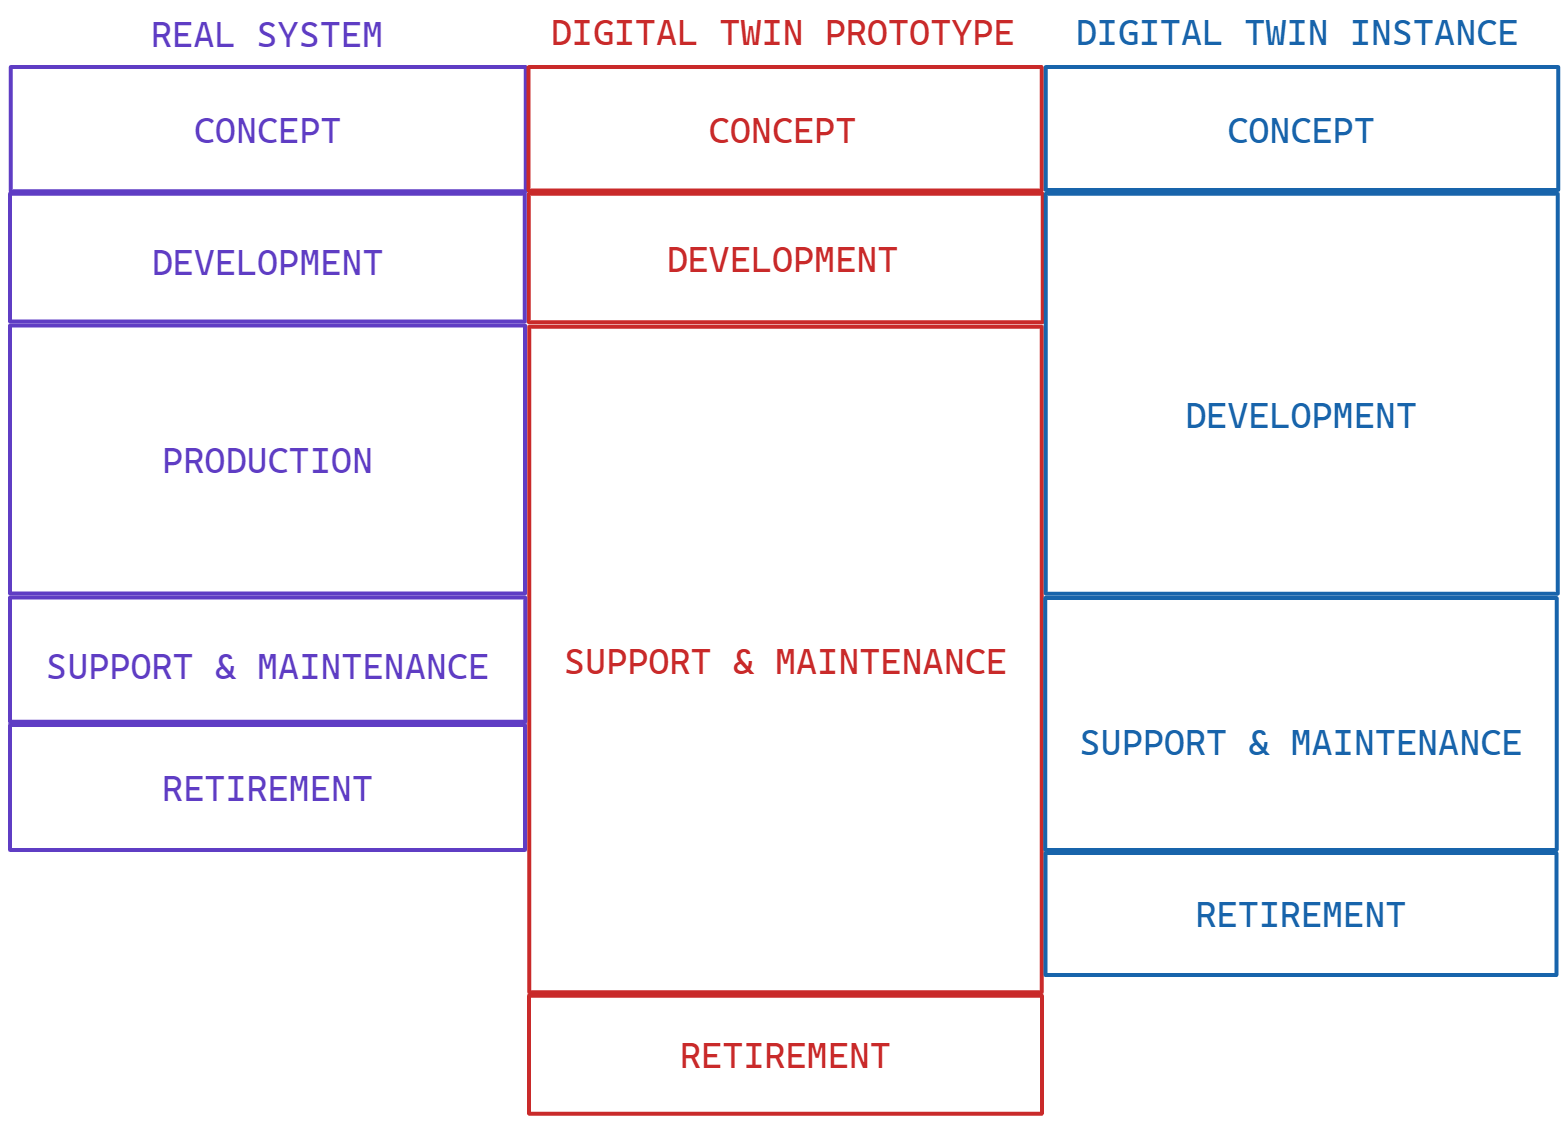
\includegraphics[width=0.45\textwidth]{LIFECYCLE.png}
        \caption{Incorrect (a) and incomplete (b) status has been demonstrated with a simplified finite state machine. Incorrectness can be observed in the behavior 
        of the machine after 2 state transitions. Incompleteness, on the other hand, can be observed in the missing state. It should be noted that, even though the second state machine is missing a 
        component, it shows the right behavior, hence it is correct.}\label{fig:LIFECYCLE}
    \end{figure}
    
    It should be noted that, in the ideal world, there would be no need for a development or a concept phase for the RS. However, currently, it is not yet feasible to completely digitalize every aspect of the real system,
    hence  DTI and DTP were used to assist the RS through its lifecycle by transforming atoms to bits /ref.

    \subsection{Concept Stage}
    The concept stage for the DTP, DTI, and RS was initiated at the same time, aimed to have initial considerations and find feasible solutions, that align with the desires of the stakeholders. Although this study was a solo project, the RS, DTP, and DTI were shown to multiple individuals, hence the use of the plural term "stakeholders" was appropriate. 

    This stage was responsible for exploration, fact-finding, and initial planning while considering the economic, technical, and strategic aspects of the system. For that reason, a fast-paced requirement 
    engineering approach was selected, which resulted in the identification of functional and quality requirements, as well as constraints for the DTP, DTI, and RS.  
    After the requirement analysis was done, the approval to proceed to the Development Stage was given. 
    
    \subsection{Development Stage}
    Similar to the concept phase, the development of the  DTP, DTI, and RS was started simultaneously. In this stage, the requirements and design solutions for each were transformed 
    into feasible products which were used in the following stages of the lifecycle. The primary objective of this stage was to create hardware and software models as well as their corresponding interfaces. 
    These created models were analyzed, verified, and validated. 



    Even though the information about the assembly and production planning, maintenance and support procedures as well as retirement considerations, and many other aspects should ideally be present 
    at this stage, they were not included in this study. 

    As a result of this stage, the RS was developed and assembled digitally within the DTE as a DTP. This DTP was prepared to assemble the physical components of the RS in the physical, observable environment.  
    After the verification and validation process of the developed RS within the DTE was finished, approval to proceed to the Production Stage was given.

    \subsection{Production Stage}
    The production stage of the RS, which was constrained by the development stage of the DTP, progressed with the assistance of  DTP in the observable environment.  As an outcome, the RS was initialized successfully in the observable world and was ready for operation during the support and maintenance stage. However, the development stage of the DTI constrained this initiation. Therefore, the development of the DTI was completed before the initiation of the support and maintenance stage of the RS.  
    Additionally, the connection between the DTI and RS was established, tested, and evaluated to ensure data capture during the operation.

    \subsection{Service and Maintenance Stage}
    After the production stage, the RS and DTI started to function together. This functionality or rather a behavior was demonstrated to both technical and non-technical individuals, 
    and this way, the usage of the system was simulated. However, the feedback and assessment from these individuals, such as the quality of the system relative to user perspective,
    was out of scope for this paper, hence they were not included.  Furthermore, since there was no need for modifications while using/operating the system, 
    as a result, maintenance considerations were excluded. As an outcome of this stage, the real system was ready to be put out of service, in other words, was ready to retire.

    \subsection{Retirement Stage}

    At this stage, the product was decommissioned and the reusable parts were collected. Simultaneously, DTI was commencing to of service state as the product retired.

    Since there was no significant waste generated, there was no need for a disposal process.  

    \section{Implementation}\label{section:implementation}

    By following the lifecycle framework in Methods, the author ended up using several hardware and software to conceptualize, develop, produce, operate, and retire the RS along with the DTI and DTP.

    First, in the concept stage the requirements were gathered, listed finally categorized into three different groups. Second these requirements were revised and elicitated into more requirements before the development stage. 
    In the development stage, these requirements were fulfilled with selected software and hardware, and the real system was developed digitally, and later integrated within the Omniverse. Next digital twin prototype behavior is written with C++ along with the Robot Operating System Nodes as a ROS2 Package. These nodes were connected to the DTE with the ROS2 Bridge, hence the behavior of the digital twin prototype against the requirements was tested, validated, and verified. 
    In the production stage, the real system was successfully assembled in the observable environment according to the digital twin prototype. Next, the digital twin prototype was copied and developed further,  to make a seamless connection between the digital twin instance and a real system. After the development of the digital twin instance was finished, the connection between the real system and the digital twin instance was tested. 
    In the support \& maintenance stage, the behavior of the real system and digital twin instance is observed by the individuals, which resulted in great feedback, which proved subjectively, the seamless connection between the real system and digital twin instance with required fidelity. 
    After the observations, the system got into the retirement stage, and the digital twin instance and later digital twin prototype were retired.

    \subsection{Implementation of the Concept Stage}
    For the concept stage, first, the author focused on the requirement analysis and gathered all the requirements for the possible system. Software such as Obsidian along with the Excalidraw community plugin was used to conceptualize the systems and most importantly 
    for the documentation of the requirements. Each system requirement was considered separately and later put together in the table. Requirements for the DTE were not considered.    

    Later, several prototyping not only digital but also partially physical prototyping was done. 
    Requirements were revised, elicitated, and reworked, which resulted in a feasible solution with the selected components to develop a digital twin prototype within the Omniverse.
    
    \begin{figure}[htbp]
        \centering
        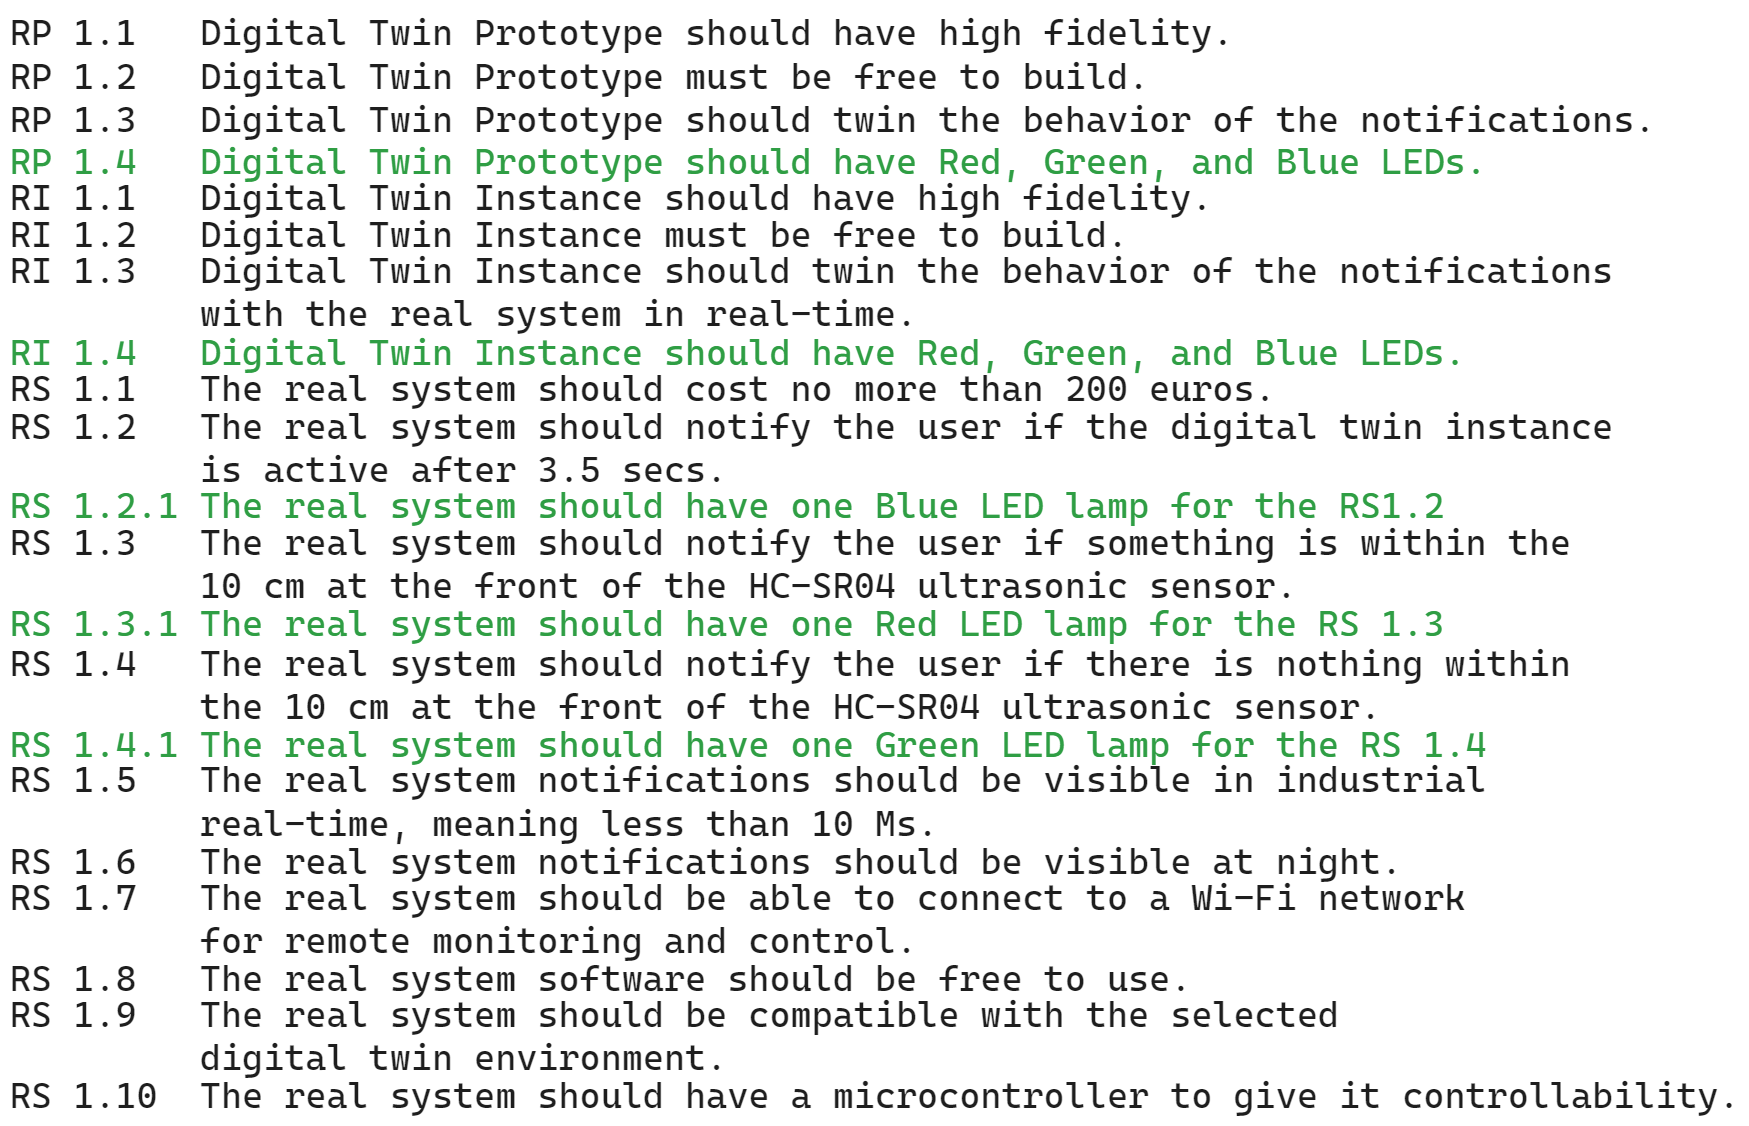
\includegraphics[width=0.55\textwidth]{Requirements.png}
        \caption{Incorrect (a) and incomplete (b) status has been demonstrated with a simplified finite state machine. Incorrectness can be observed in the behavior 
        of the machine after 2 state transitions. Incompleteness, on the other hand, can be observed in the missing state. It should be noted that, even though the second state machine is missing a 
        component, it shows the right behavior, hence it is correct.}\label{fig:Requirements}
    \end{figure}

    \subsection{Implementation of the Development Stage}
    After these requirements, the development of the DTP was started. To create a DTP of the planned RS, two different software programs were used for two different purposes including Fusion 360, 
    a Computer-Aided Design software, and Blender, a 3D-Graphics software. Later the modeled DTP is integrated into the Omniverse, and the behavior is given with the ROS2 node.

    First, pre-existing digitalized possible RS components were sourced from the internet, and modified for use. The ones that were not found, such as jumper cables, were developed by the author 
    in the Fusion 360. Once all the required components were available and the model reached the required fidelity level, detailing was stopped and parts were digitally assembled. 
    Lastly, the assembled digital model was converted to a .fbx file.

    After the conversion, the Blender was used, to convert a .fbx file to a .usd file for the intention of importing into the DTE. However, before the conversion, 
    adjustments were made to the .fbx file to fix issues, such as corrupted visuals and inherited hierarchy problems, which occurred due to the insufficient performance of the conversion. 
    Later, the corrected file was converted into a .usd file. 

    Finally, Blender was reopened, and the previously converted .usd file was imported. Further adjustments were made to the file and were saved again as a .usd file. Upon completion of this process, 
    the file was prepared for importation into the DTE.

    Furthermore, headless Ubuntu 20.04 was installed on a micro-SD card, and inserted into the RPI4. Second, the cryptographic network protocol SSH was used to connect the RPI4 to a local computer that already had Ubuntu 20.04.
     Subsequently, the Robot Operating System 2 (ROS2) version of Foxy was installed on both the RPI 4 and the local computer. 
     Lastly, to access and control the GPIO pins of the RPI4, the Wiring Pi library was installed on RPI4.

    ROS2 was used as a sensor and communication middleware to give behavior to the real system components as well as to digital twin instances. 
    Therefore, a custom package was developed with C++  to read data from the ultrasonic sensor and control the state of three LEDs. This behavior was integrated into a single node, which was executed with a single-thread executor. Lastly, the combined ROS2 node was run, and the required behavior of the real system was observed in the digital twin prototype to ensure that the three LEDs were giving the possible state of the RS.

    The chosen DTE for this demonstration was Isaac Sim, which is fully integrated into the NVIDIA Omniverse platform. Isaac Sim was designed specifically for the training and testing of complex robotic 
    systems in realistic virtual environments. Despite the simplicity of the demonstration, which was not a complex robotic system, there were two crucial reasons for the platform selection. 
    First, Isaac Sim offers a ROS2 bridge, which enabled a seamless connection between ROS2 and Omniverse, facilitating relatively easy and smooth data exchange. Second, it leverages RTX Graphics, 
    which delivered high-performance graphics rendering, resulting in an improvement in visual fidelity. 

    First, to initialize the DTE, Isaac Sim was installed on a local computer using the Omniverse launcher. Once the installation was completed, the correct ROS2 bridge was selected. 
    At this step, it was important not to source the ROS2 Workspace within the same terminal that Isaac Sim was operating, for example with the automatic sourcing via bashrc, to prevent potential compilation errors. 

    After the initialization, the modified .usd file was imported into the Isaac Sim scene. After the import, a visual inspection of the individual 
    parts was then conducted, and needed adjustments were made. 

    Next, to integrate the behavior, visual scripting has been used with the integrated ROS2 bridge, which resulted in the integrated behavior. 
    Later behavior of the LEDs was tested, and needed corrections have been made. As a consequence, the required level of fidelity of the DTP, within the DTE 
    was reached successfully, and the next step, which was the assembly of the real system was ready.

    
    \begin{figure}[htbp]
        \centering
        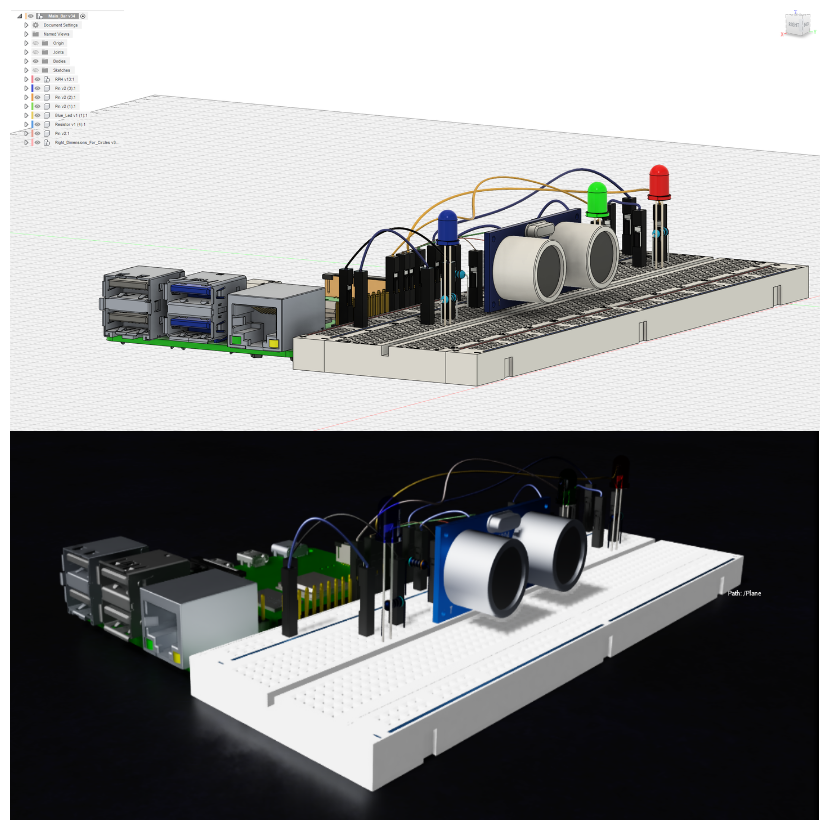
\includegraphics[width=0.5\textwidth]{Left.png}
        \caption{Incorrect (a) and incomplete (b) status has been demonstrated with a simplified finite state machine. Incorrectness can be observed in the behavior 
        of the machine after 2 state transitions. Incompleteness, on the other hand, can be observed in the missing state. It should be noted that, even though the second state machine is missing a 
        component, it shows the right behavior, hence it is correct.}\label{fig:Left}
    \end{figure}

    \subsection{Implementation of the Production Stage}
    First, the components were assembled on the prototype breadboard in accordance with the DTP. Next, circuit components were connected with the jumper cables to the appropriate general-purpose input/output (GPIO), ground, and power pins of Raspberry Pi 4 (RPI4). 

    After the assembly, the DTI interfaces were developed and the ROS2 node from the DTP was copied and later modified, to connect the RS to the DTI. It should be noted that only the behavior of the LEDs was twinned and not the other attributes of the RS such as spatial data of the components were not. This connection was tested visually. 

    After the development of the DTI was finalized, the RS was ready to proceed to the operation in the support and maintenance stage.

    \begin{figure}[htbp]
        \centering
        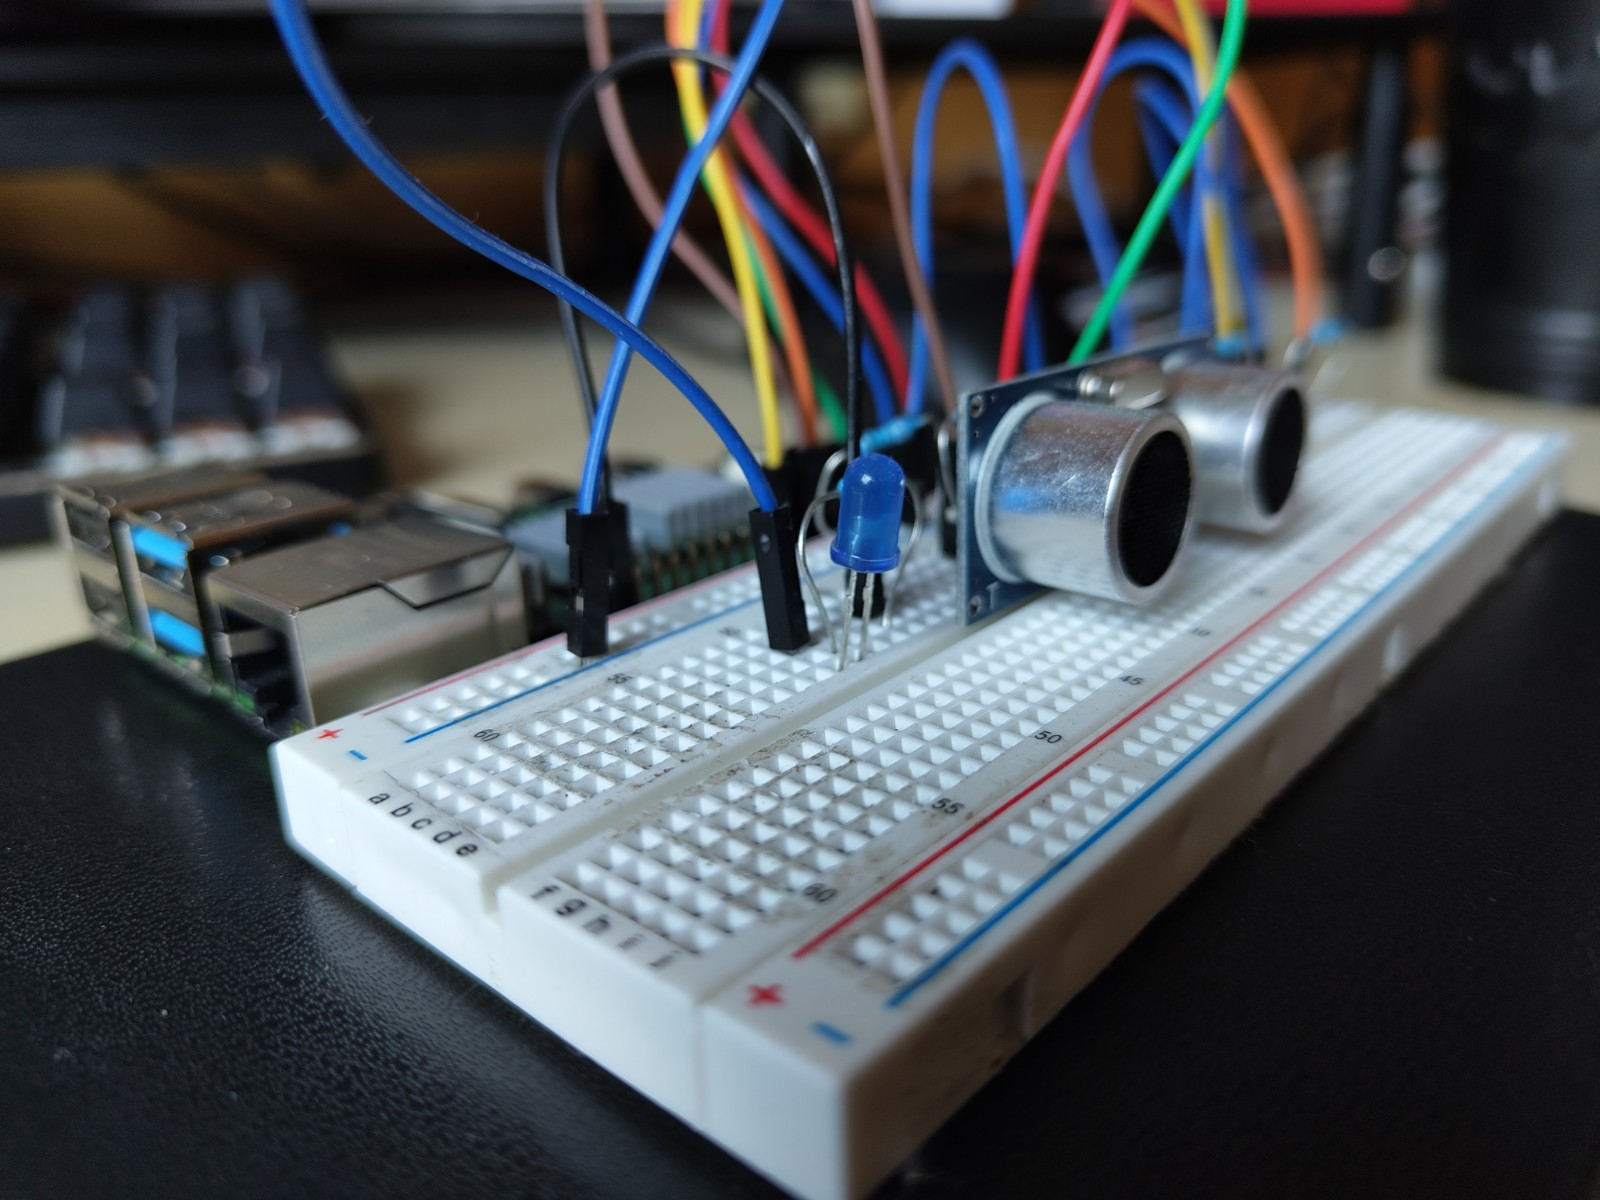
\includegraphics[width=0.5\textwidth]{Assembled.jpg}
        \caption{Incorrect (a) and incomplete (b) status has been demonstrated with a simplified finite state machine. Incorrectness can be observed in the behavior 
        of the machine after 2 state transitions. Incompleteness, on the other hand, can be observed in the missing state. It should be noted that, even though the second state machine is missing a 
        component, it shows the right behavior, hence it is correct.}\label{fig:Assembled}
    \end{figure}

    \subsection{Implementation of the Support and Maintenance Stage}
    RS, DTI, and DTP were shown to the stakeholders and their assessment of the quality attributes was written. After all, stakeholders saw the RS, DTI, and DTP, the RS was ready to be decommissioned with the corresponding DTI.
    
    \subsection{Implementation of the Retirement Stage}
    The RS was decommissioned and disassembled, and the DTI was achieved with it. DTP is also archived, however, with the many products, that would not be the case.

    \section{Observations} 
    To address the challenges associated with the accessibility and comprehensibility of the notion of digital twins, authors followed a lifecycle model to present the lifecycle stages of an RS, with the DTI and DTP.During these stages, there were some observations, and challenges during the process of creating the digital twins. 
    
    \subsection{Observations while Creating Digital Twin Prototype}

    First, the authors did not consider the CAD environment as a digital environment, instead considered Omniverse as a digital environment. Therefore, in this application, conversion of CAD files to .obj or .fbx and later to .usd was inevitable. The results of the conversions show that a significant amount of model data gets lost, corrupted, or duplicated during the file conversions because of the complexity of the models. Therefore to minimize the data loss, reducing the number of parts by grouping parts together as one solid part and removing the unnecessary details, modifying the names of the parts to simple ones, and deleting material properties were helpful and needed. However, some of these processes are irreversible, hence they might reduce the fidelity of the model drastically.

    Further observations show that, during the modeling process, non-conventional ways, such as modeling electric cables as 3D in CAD, increased the overall fidelity of the DTP and consequently.

    Lastly, there was a significant difference in data loss, due to the quality of file converters, Blender and Embedded Omniverse Converter, when the conversion of the .fbx file to a .usd file was wanted. Hence, before putting the .fbx file directly into the omniverse, putting it into the blender and modifying there,  gives a better conversion of .fbx to .usd as well as gives more flexibility to manipulate the corrupted data which occurs during the conversion to .fbx file from .step file.

    \subsection{Observations while creating a real system}

    First, the assembly time of the real system according to the digital model, dramatically decreased, due to the provided spatial and visual data from the digital model, especially the cabling between the RPI and the breadboard. 

    Also the safety of components, during the assembly, also increased, which prevented common mistakes such as giving higher voltage to GPIO pins, which could result in damaging the RPI, was prevented. 

    \subsection{Observation while creating a DTI}

    The evolvability of the DTP is important, which reduces the development time of the DTI drasticaly. For example, pre-defined interfaces while developing the DTP, would be really helpful to develop the DTI. In ideal case, the whole DTP could be used as a template, if the DTP is adjustable, hence evolvable. 

    \subsection{Observation while operating the DTI}

    Even though, the behavior of the LEDs were correctly twinned, the other information about the LEDs such as spatial data was missing which resulted in incorrect ideal twinning process. For example, removing the LED from the circuit was not presented in the digital twin instance. For this representation, it was not an issue, because in the requirements of the DTI and DTP that was not a required statement, however for the industrial applications it should be considered, and can be done with the machine vision. 

    \section{Conclusion}

    Digital twins as a notion, a powerful tool or rather approach to support(or even replace) the lifecycle stages of the product, which helps to reduce the needed material, energy, and time by using the information, which is acquired by the digital twin of the product. 

    With the help of new technologies and approaches, such as machine learning, IoT, VR/AR, Robotics, and Automation,  the information about the product can be exploited even in much more depth, which results in better DTP's and DTI's. However, until today, there isn't a standardized framework, which shows how this exploitation should be handled. Such challenges, Cybersecurity, data integration, model accuracy, and model calibration are adding up to the standardization problem. Consequently, more research and development should be made for the digital twins, to implement and trade the information with the needed material, energy, and time. 

    Questions such as Is the DTI just the evolution of the DTP or is it another entity?, How can the quality of the DTI's as well as DTP's be qualified? Is the lifecycle of the product can be fully replaceable by the DTI and DTP? How to standardize the DTP and DTI? What is the lifecycle of the DTI and DTP?  can be researched further.
    \bibliography{main}
    \bibliographystyle{plain}
    
\end{document}